%
%INÍCIO DO PREÂMBULO
%

\documentclass[mscexam,numbers]{coppe}
%Pacotes padrão do CoppeTeX
\usepackage{amsmath,amssymb}
%Pacote Hyperref já usado mais abaixo com mais opções
%\usepackage{hyperref}

%Usando fonte semelhante à Times New Roman
\usepackage[T1]{fontenc}
\usepackage{tgtermes}

\makelosymbols
\makeloabbreviations

%Criando modo de inserir lista específica de gráficos
\usepackage{caption}
\DeclareCaptionType{grafico}[Gráfico][Lista de Gráficos]

%Criando modo de inserir lista específica de quadros
\DeclareCaptionType{quadro}[Quadro][Lista de Quadros]

%Substituindo "Capítulo X" no início de cada capítulo pelo nome do capítulo
\usepackage{titlesec}
%\titleformat{\chapter}[hang]{\bf\huge}{\thechapter}{2pc}{}
%\titlespacing*{\chapter}{0pt}{-50pt}{40pt}

%Removendo o espaçamento extra antes do início de cada capítulo
\titleformat{\chapter}[display]
{\normalfont\huge\bfseries}{\chaptertitlename\ \thechapter}{20pt}{\Huge}
\titlespacing*{\chapter}{0pt}{-50pt}{40pt}

%Adicionando numeração ao nível 4, 5 e 6:1.1.1.1, 1.1.1.1.1 e 1.1.1.1.1.1
\addtocounter{secnumdepth}{3}

%Adicionando epígrafes
\usepackage{epigraph}
%Removendo o traço horizontal default da epígrafe
\setlength{\epigraphrule}{0pt}

%Adicionando o campo "fonte" nas ilustrações
\newcommand{\source}[1]{\caption*{Fonte: {#1}} }

%Adicionando apêndices de uma forma melhor
\usepackage[titletoc]{appendix}

%Melhorando a qualidade do Sumário
\makeatletter
\renewcommand*\l@chapter[2]{%
  \ifnum \c@tocdepth >\m@ne
    \addpenalty{-\@highpenalty}%
    \vskip 1.0em \@plus\p@
    \setlength\@tempdima{1.5em}%
    \begingroup
      \parindent \z@ \rightskip \@pnumwidth
      \parfillskip -\@pnumwidth
      \leavevmode \bfseries
      \advance\leftskip\@tempdima
      \hskip -\leftskip
      #1\nobreak
      \xleaders\hbox{$\m@th
        \mkern \@dotsep mu\hbox{.}\mkern \@dotsep
        mu$}\hfill%
      \nobreak\hb@xt@\@pnumwidth{\hss #2}\par
      \penalty\@highpenalty
    \endgroup
  \fi}
\renewcommand*\l@section{\@dottedtocline{1}{1.5em}{2.3em}}
\renewcommand*\l@subsection{\@dottedtocline{2}{3.8em}{3.2em}}
\renewcommand*\l@subsubsection{\@dottedtocline{3}{7.0em}{4.1em}}
\renewcommand*\l@paragraph{\@dottedtocline{4}{10em}{5em}}
\renewcommand*\l@subparagraph{\@dottedtocline{5}{12em}{6em}}
\makeatother

%Adicionando suporte para ilustrações que ocupam a página toda em modo paisagem
\usepackage{pdflscape}

%Adicionando suporte para tabelas espalhando-se por múltiplas páginas
\usepackage{longtable}

%Adicionando capacidade de referência e referência invertida em todo o documento
\usepackage[backref=page]{hyperref}
\def\backref#1{{\scriptsize [#1]}}

%Adicionando índice remissivo no documento
\usepackage{makeidx}
\makeindex

%Inserir como padrão a indentação do primeiro parágrafo de cada capítulo, que na língua inglesa não é o caso, porém na portuguesa é
%Não altera nada para capítulos com epígrafe
\usepackage{indentfirst}

%
%
%FIM DO PREÂMBULO
%
%
%

\begin{document}
  %Todo necessario para a criação dos seguintes elementos pré-textuais:
  %1 Folha de rosto
  %2 Folha de aprovação
  %3 Ficha catalográfica
  \title{Educação empreendedora nas escolas de engenharia: uma revisão sistemática da literatura}
  \foreigntitle{Entrepreneurial education at engineering schools: a systematic literature review}
  \author{Bruno}{Campana}
  \advisor{Prof.}{Édison Renato Pereira da}{Silva}{D.Sc.}

  \examiner{Prof.}{Édison Renato Pereira da Silva}{D.Sc.}
  \examiner{Prof.}{Domício Proença Júnior}{D.Sc.}

  \department{PEP}
  \date{03}{2022}

  \keyword{engineering education}
  \keyword{entrepreneurial education}
  \keyword{entrepreneurial engineering}

  \maketitle
  
  \providecommand\frontmatter

  %ajustar!
  \dedication{Dedicado à minha linda esposa.}

  \chapter*{Agradecimentos}
Gostaria de agradecer a todos.


  \begin{abstract}
	
  O bitcoin é a primeira moeda descentralizada do mundo. Isso significa que, além de não ser regulado por governos, bancos ou empresas, é possível comprar, enviar e receber bitcoins sem nenhum intermediário, como bancos ou emissores de cartão de crédito. 
  
  Além disso, é uma moeda limitada. Diferentemente do real, dólar e euro, moedas que podem ser emitidas conforme os países sentirem necessidade, o bitcoin e seu código foram criados de forma que somente 21 milhões de moedas possam ser emitidas – este é o limite. Até 2019, estima-se que 18 milhões de bitcoins já haviam sido emitidos.
\end{abstract}


  \begin{foreignabstract}

Bitcoin (BTC) is a cryptocurrency, a virtual currency designed to act as money and a form of payment outside the control of any one person, group, or entity, thus removing the need for third-party involvement in financial transactions. It is rewarded to blockchain miners for verifying transactions and can be purchased on several exchanges.

\end{foreignabstract}


  \tableofcontents
  %\listoffigures
  {%
    \let\oldnumberline\numberline%
    \renewcommand{\numberline}{\figurename~\oldnumberline}%
    \listoffigures%
  }
  {%
    \let\oldnumberline\numberline%
    \renewcommand{\numberline}{\tablename~\oldnumberline}%
    \listoftables%
  }
  %\listoftables
  %\listofgraficos
  {%
    \let\oldnumberline\numberline%
    \renewcommand{\numberline}{\graficoname~\oldnumberline}%
    \listofgraficos%
  }
  %\listofquadros
  {%
    \let\oldnumberline\numberline%
    \renewcommand{\numberline}{\quadroname~\oldnumberline}%
    \listofquadros%
  }
  \printlosymbols
  \printloabbreviations

  \mainmatter

  \chapter{Introdu{\c c}\~ao}

\epigraph{\textit{Subindo nos ombros de gigantes.}}{--- Isaac Newton}

Primeiro de tudo precisa ser definido o que é a engenharia \index{engenharia}.

Segundo a norma de formata{\c c}\~ao de teses e disserta{\c c}\~oes do
Instituto Alberto Luiz Coimbra de P\'os-gradua{\c c}\~ao e Pesquisa de
Engenharia (COPPE), toda abreviatura deve ser definida antes de
utilizada.\abbrev{COPPE}{Instituto Alberto Luiz Coimbra de P\'os-gradua{\c
c}\~ao e Pesquisa de Engenharia}

Do mesmo modo, \'e imprescind\'ivel definir os s\'imbolos, tal como o
conjunto dos n\'umeros reais $\mathbb{R}$ e o conjunto vazio $\emptyset$.
\symbl{$\mathbb{R}$}{Conjunto dos n\'umeros reais}
\symbl{$\emptyset$}{Conjunto vazio}

\begin{longquote}
Um exemplo de citação longa nas regras da ABNT (4cm de recuo e fonte menor)
feita com o ambiente  \verb=longquote= The primary objective of this
investigation was to determine the feasibility of detecting corrosion in
aluminum Naval aircraft components with neutron radiographic interrogation
and the use of standard corrosion penetrameters. Secondary objectives
included the determination of the effect of object thickness on image quality,
the defining of minimum levels of detectability and a preliminary investigation
of a means whereby the degree of corrosion could be quantified with neutron
radiographic data. \cite{article-example}
\end{longquote}

Agora vamos testar o uso de abreviações, com uma que aparecerá muitas vezes ao longo do texto: RSL (Revisão Sistemática da Literatura). \abbrev{RSL}{Revisão Sistemática da Literatura}. Otorrinolaringologista, Otorrinolaringologista, Otorrinolaringologista, Otorrinolaringologista, Otorrinolaringologista, Otorrinolaringologista,Otorrinolaringologista, Otorrinolaringologista, Otorrinolaringologista, Otorrinolaringologista, Otorrinolaringologista, Otorrinolaringologista, Otorrinolaringologista, Otorrinolaringologista, Otorrinolaringologista, Otorrinolaringologista,Otorrinolaringologista, Otorrinolaringologista, Otorrinolaringologista, Otorrinolaringologista, Otorrinolaringologista, Otorrinolaringologista, Otorrinolaringologista, Otorrinolaringologista, Otorrinolaringologista, Otorrinolaringologista,Otorrinolaringologista, Otorrinolaringologista, Otorrinolaringologista, Otorrinolaringologista, Otorrinolaringologista, Otorrinolaringologista, Otorrinolaringologista, Otorrinolaringologista, Otorrinolaringologista, Otorrinolaringologista,Otorrinolaringologista, Otorrinolaringologista, Otorrinolaringologista, Otorrinolaringologista, Otorrinolaringologista, Otorrinolaringologista, Otorrinolaringologista, Otorrinolaringologista, Otorrinolaringologista, Otorrinolaringologista,Otorrinolaringologista, Otorrinolaringologista, Otorrinolaringologista, Otorrinolaringologista, Otorrinolaringologista, Otorrinolaringologista, Otorrinolaringologista, Otorrinolaringologista, Otorrinolaringologista, Otorrinolaringologista,Otorrinolaringologista,

\begin{figure}[!hbt]
  \centering
  \caption{Uma figura de exemplo}
  \makebox[0pt]{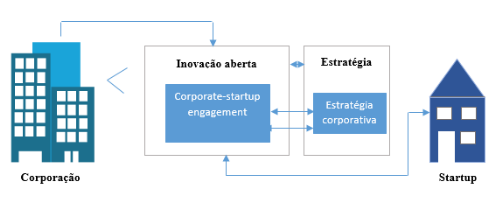
\includegraphics[]{Figuras/figura-exemplo}}
  \source{Elaborado pelo autor}
  \label{figura-exemplo}
\end{figure}

Otorrinolaringologista, Otorrinolaringologista, Otorrinolaringologista, Otorrinolaringologista, Otorrinolaringologista, Otorrinolaringologista, Otorrinolaringologista, Otorrinolaringologista, Otorrinolaringologista,Otorrinolaringologista, Otorrinolaringologista, Otorrinolaringologista, Otorrinolaringologista, Otorrinolaringologista, Otorrinolaringologista, Otorrinolaringologista, Otorrinolaringologista, Otorrinolaringologista, Otorrinolaringologista,Otorrinolaringologista, Otorrinolaringologista, Otorrinolaringologista, Otorrinolaringologista, Otorrinolaringologista, Otorrinolaringologista, Otorrinolaringologista, Otorrinolaringologista, Otorrinolaringologista, Otorrinolaringologista,Otorrinolaringologista, Otorrinolaringologista, Otorrinolaringologista, Otorrinolaringologista, Otorrinolaringologista, Otorrinolaringologista, Otorrinolaringologista, Otorrinolaringologista, Otorrinolaringologista, Otorrinolaringologista,Otorrinolaringologista, Otorrinolaringologista, Otorrinolaringologista, Otorrinolaringologista, Otorrinolaringologista, Otorrinolaringologista, Otorrinolaringologista, Otorrinolaringologista, Otorrinolaringologista, Otorrinolaringologista,Otorrinolaringologista, Otorrinolaringologista, Otorrinolaringologista, Otorrinolaringologista, Otorrinolaringologista, Otorrinolaringologista, Otorrinolaringologista, Otorrinolaringologista, Otorrinolaringologista, Otorrinolaringologista,Otorrinolaringologista, Otorrinolaringologista, Otorrinolaringologista, Otorrinolaringologista, Otorrinolaringologista, Otorrinolaringologista, Otorrinolaringologista, Otorrinolaringologista, Otorrinolaringologista, Otorrinolaringologista,Otorrinolaringologista, Otorrinolaringologista, Otorrinolaringologista, Otorrinolaringologista, Otorrinolaringologista, Otorrinolaringologista, Otorrinolaringologista, Otorrinolaringologista, Otorrinolaringologista, Otorrinolaringologista,Otorrinolaringologista, Otorrinolaringologista, Otorrinolaringologista, Otorrinolaringologista, Otorrinolaringologista, Otorrinolaringologista, Otorrinolaringologista, Otorrinolaringologista, Otorrinolaringologista, Otorrinolaringologista,Otorrinolaringologista, Otorrinolaringologista, Otorrinolaringologista, Otorrinolaringologista.

\begin{grafico}[!hbt]
  \centering
  \caption{Um gráfico de exemplo}
  \makebox[0pt]{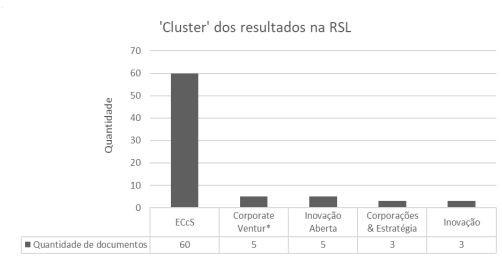
\includegraphics[]{Gráficos/grafico-exemplo}}
  \source{Elaborado pelo autor}
  \label{grafico-exemplo}
\end{grafico}


  \chapter{Revis\~ao Bibliogr\'afica}

Para ilustrar a completa ades\~ao ao estilo de cita{\c c}\~oes e listagem de
refer\^encias bibliogr\'aficas, a Tabela~\ref{tab:citation} apresenta cita{\c
c}\~oes de alguns dos trabalhos contidos na norma fornecida pela CPGP da
COPPE, utilizando o estilo num\'erico.

\begin{table}[h]
\caption{Exemplos de cita{\c c}\~oes utilizando o comando padr\~ao
  \texttt{\textbackslash cite} do \LaTeX\ e
  o comando \texttt{\textbackslash citet},
  fornecido pelo pacote \texttt{natbib}.}
\label{tab:citation}
\centering
{\footnotesize
\begin{tabular}{|c|c|c|}
  \hline
  Tipo da Publica{\c c}\~ao & \verb|\cite| & \verb|\citet|\\
  \hline
  Livro & \cite{book-example} & \citet{book-example}\\
  Artigo & \cite{article-example} & \citet{article-example}\\
  Relat\'orio & \cite{techreport-example} & \citet{techreport-example}\\
  Relat\'orio & \cite{techreport-exampleIn} & \citet{techreport-exampleIn}\\
  Anais de Congresso & \cite{inproceedings-example} &
    \citet{inproceedings-example}\\
  S\'eries & \cite{incollection-example} & \citet{incollection-example}\\
  Em Livro & \cite{inbook-example} & \citet{inbook-example}\\
  Disserta{\c c}\~ao de mestrado & \cite{mastersthesis-example} &
    \citet{mastersthesis-example}\\
  Tese de doutorado & \cite{phdthesis-example} & \citet{phdthesis-example}\\
  \hline
\end{tabular}}
\end{table}


  \chapter{Design da Pesquisa}

\section{Nível 2}
And taking advantage of the quote from Satoshi Nakamoto, there are also those who say: "Bitcoin was not supposed to be like that. This is not what Satoshi Nakamoto conceived". Note, I don't know what exactly the individual or group behind the Bitcoin invention conceived. But you see, every human invention encapsulates the knowledge and knowhow of its creator. Encapsulate your ideas. But after "free in the world", invention has a "life of its own", and the ecosystem that was created from the invention has a life of its own. For good and for bad. There is not much more to be said for this.

We are near the end of the opinions I would like to express. One of the last concerns the opinions of politicians, investors, bankers and researchers about the future potential for cryptocurrencies. As I've already expressed, I see no reason to treat cryptocurrencies as an innovation unlike any other technological advance seen in humanity. And so, I am optimistic about the potential of cryptocurrencies, but realistic, far from the detachment from reality of some "moon boys". Now, one of the nuisances driving the perceived value of cryptocurrencies up is good news coming from these industries, which is fair, because it implies progress in adoption. On the other hand, there is the impact of bad news also coming from politicians, investors, bankers and researchers. And it is on this news that I want to do one of our latest mental exercises.

\subsection{Nível 3}
These people, sometimes representatives of large organizations, are ultimately the guardians of the status quo, for better or for worse. The opinions they declare, therefore, never define the true disruptive potential of cryptocurrencies, but rather the position that public opinion is wanted to believe on the subject. What do you expect to hear, for example, in an interview with, for example, an FED director? Do you think it's possible that he'll say something like: "Cryptocurrencies are indeed disruptive, they have enormous potential to transform the current financial system, and it's all a shame, because the organization I represent tends to lose more and more relevance because of it. of that and we will also lose the monopoly of issuing fiat money". Do you really think that a representative of the status quo, public or private, will say something like this?

Representatives of the status quo will always present opinions in defense of the status quo. It doesn't matter which arguments are used. The arguments will sometimes be good, sometimes bad, but the purpose behind is always to maintain the status quo. Simultaneously with any attempt to maintain the status quo, there are organizations that perceive change as an opportunity to uplift the current status quo, that is, to turn innovation into a competitive differential for themselves. These organizations can be companies or even countries, and in the case of cryptocurrencies, they can see: "Ok, I'm going to dive into cryptocurrencies, because I can make this a competitive advantage for my country."

\subsubsection{Nivel 4}
It is a natural scenario, inherent to any major transformation in society, markets, form and type of goods and services provided. The point is: bullish news about crypto adoption is indeed bullish news. But you have to be careful with pessimistic news, because deep down, from the beginning, you never expected anything different after all. Organizations that find themselves in a position of dominance of the current status quo, in control of the financial system, will only take positive moves in favor of cryptocurrencies to avoid a "greater evil" from falling behind in relation to other organizations that adopt cryptos as a competitive differential.

And as a last reflection, I invite you to the following reflection: how wrong can all this go? Could it be that all the disruptive potential of cryptocurrencies hasn't already been priced in, and haven't we gone much further? This question is very pertinent. The most pertinent for the cryptocurrency investor after all. The "moon boys" want us to believe that "there are no limits", but in my opinion, there is a limit. Although the adoption of cryptos by society occurs extremely quickly and painlessly, without the need for a "war" against the current status quo, even if the entire world economic system is transformed, there are still limits to the intrinsic and extrinsic value of the sector. Remember the economy is bigger than that.

\paragraph{Nível 5}
Judging by the innovations that cryptocurrencies are likely to bring, I believe there is still room for investment in the sector, without it being detached from the real potential of generating value to society. And I believe this because, a lot is said about cryptoCURRENCY, but beyond that, the central point here is not the money, but the transactions. And transactions aren't just economical. Every exchange of information in social dynamics is a transaction. The combination of cryptography with a decentralized consensus protocol undoubtedly finds its greatest utility in the financial system, but it is far from being the last. Ultimately, a decentralized consensus protocol is likely to change the dynamics of the entire internet as we know it today. This is definitely not a small thing, and it is definitely not of little value.

\subparagraph{Nível 6}
And taking advantage of the quote from Satoshi Nakamoto, there are also those who say: "Bitcoin was not supposed to be like that. This is not what Satoshi Nakamoto conceived". Note, I don't know what exactly the individual or group behind the Bitcoin invention conceived. But you see, every human invention encapsulates the knowledge and knowhow of its creator. Encapsulate your ideas. But after "free in the world", invention has a "life of its own", and the ecosystem that was created from the invention has a life of its own. For good and for bad. There is not much more to be said for this.

We are near the end of the opinions I would like to express. One of the last concerns the opinions of politicians, investors, bankers and researchers about the future potential for cryptocurrencies. As I've already expressed, I see no reason to treat cryptocurrencies as an innovation unlike any other technological advance seen in humanity. And so, I am optimistic about the potential of cryptocurrencies, but realistic, far from the detachment from reality of some "moon boys". Now, one of the nuisances driving the perceived value of cryptocurrencies up is good news coming from these industries, which is fair, because it implies progress in adoption. On the other hand, there is the impact of bad news also coming from politicians, investors, bankers and researchers. And it is on this news that I want to do one of our latest mental exercises.

These people, sometimes representatives of large organizations, are ultimately the guardians of the status quo, for better or for worse. The opinions they declare, therefore, never define the true disruptive potential of cryptocurrencies, but rather the position that public opinion is wanted to believe on the subject. What do you expect to hear, for example, in an interview with, for example, an FED director? Do you think it's possible that he'll say something like: "Cryptocurrencies are indeed disruptive, they have enormous potential to transform the current financial system, and it's all a shame, because the organization I represent tends to lose more and more relevance because of it. of that and we will also lose the monopoly of issuing fiat money". Do you really think that a representative of the status quo, public or private, will say something like this?

Representatives of the status quo will always present opinions in defense of the status quo. It doesn't matter which arguments are used. The arguments will sometimes be good, sometimes bad, but the purpose behind is always to maintain the status quo. Simultaneously with any attempt to maintain the status quo, there are organizations that perceive change as an opportunity to uplift the current status quo, that is, to turn innovation into a competitive differential for themselves. These organizations can be companies or even countries, and in the case of cryptocurrencies, they can see: "Ok, I'm going to dive into cryptocurrencies, because I can make this a competitive advantage for my country."

It is a natural scenario, inherent to any major transformation in society, markets, form and type of goods and services provided. The point is: bullish news about crypto adoption is indeed bullish news. But you have to be careful with pessimistic news, because deep down, from the beginning, you never expected anything different after all. Organizations that find themselves in a position of dominance of the current status quo, in control of the financial system, will only take positive moves in favor of cryptocurrencies to avoid a "greater evil" from falling behind in relation to other organizations that adopt cryptos as a competitive differential.

And as a last reflection, I invite you to the following reflection: how wrong can all this go? Could it be that all the disruptive potential of cryptocurrencies hasn't already been priced in, and haven't we gone much further? This question is very pertinent. The most pertinent for the cryptocurrency investor after all. The "moon boys" want us to believe that "there are no limits", but in my opinion, there is a limit. Although the adoption of cryptos by society occurs extremely quickly and painlessly, without the need for a "war" against the current status quo, even if the entire world economic system is transformed, there are still limits to the intrinsic and extrinsic value of the sector. Remember the economy is bigger than that.

Judging by the innovations that cryptocurrencies are likely to bring, I believe there is still room for investment in the sector, without it being detached from the real potential of generating value to society. And I believe this because, a lot is said about cryptoCURRENCY, but beyond that, the central point here is not the money, but the transactions. And transactions aren't just economical. Every exchange of information in social dynamics is a transaction. The combination of cryptography with a decentralized consensus protocol undoubtedly finds its greatest utility in the financial system, but it is far from being the last. Ultimately, a decentralized consensus protocol is likely to change the dynamics of the entire internet as we know it today. This is definitely not a small thing, and it is definitely not of little value.

\begin{quadro}[!hbt]
  \centering
  \caption{Um quadro de exemplo}
  \makebox[0pt]{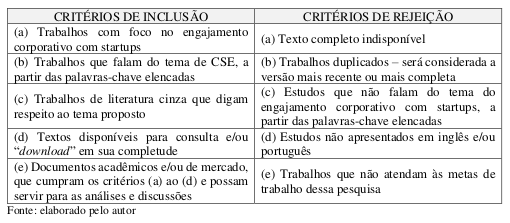
\includegraphics[]{Quadros/quadro-exemplo}}
  \source{Elaborado pelo autor}
  \label{quadro-exemplo}
\end{quadro}

And taking advantage of the quote from Satoshi Nakamoto, there are also those who say: "Bitcoin was not supposed to be like that. This is not what Satoshi Nakamoto conceived". Note, I don't know what exactly the individual or group behind the Bitcoin invention conceived. But you see, every human invention encapsulates the knowledge and knowhow of its creator. Encapsulate your ideas. But after "free in the world", invention has a "life of its own", and the ecosystem that was created from the invention has a life of its own. For good and for bad. There is not much more to be said for this.

We are near the end of the opinions I would like to express. One of the last concerns the opinions of politicians, investors, bankers and researchers about the future potential for cryptocurrencies. As I've already expressed, I see no reason to treat cryptocurrencies as an innovation unlike any other technological advance seen in humanity. And so, I am optimistic about the potential of cryptocurrencies, but realistic, far from the detachment from reality of some "moon boys". Now, one of the nuisances driving the perceived value of cryptocurrencies up is good news coming from these industries, which is fair, because it implies progress in adoption. On the other hand, there is the impact of bad news also coming from politicians, investors, bankers and researchers. And it is on this news that I want to do one of our latest mental exercises.

These people, sometimes representatives of large organizations, are ultimately the guardians of the status quo, for better or for worse. The opinions they declare, therefore, never define the true disruptive potential of cryptocurrencies, but rather the position that public opinion is wanted to believe on the subject. What do you expect to hear, for example, in an interview with, for example, an FED director? Do you think it's possible that he'll say something like: "Cryptocurrencies are indeed disruptive, they have enormous potential to transform the current financial system, and it's all a shame, because the organization I represent tends to lose more and more relevance because of it. of that and we will also lose the monopoly of issuing fiat money". Do you really think that a representative of the status quo, public or private, will say something like this?

Representatives of the status quo will always present opinions in defense of the status quo. It doesn't matter which arguments are used. The arguments will sometimes be good, sometimes bad, but the purpose behind is always to maintain the status quo. Simultaneously with any attempt to maintain the status quo, there are organizations that perceive change as an opportunity to uplift the current status quo, that is, to turn innovation into a competitive differential for themselves. These organizations can be companies or even countries, and in the case of cryptocurrencies, they can see: "Ok, I'm going to dive into cryptocurrencies, because I can make this a competitive advantage for my country."

It is a natural scenario, inherent to any major transformation in society, markets, form and type of goods and services provided. The point is: bullish news about crypto adoption is indeed bullish news. But you have to be careful with pessimistic news, because deep down, from the beginning, you never expected anything different after all. Organizations that find themselves in a position of dominance of the current status quo, in control of the financial system, will only take positive moves in favor of cryptocurrencies to avoid a "greater evil" from falling behind in relation to other organizations that adopt cryptos as a competitive differential.

And as a last reflection, I invite you to the following reflection: how wrong can all this go? Could it be that all the disruptive potential of cryptocurrencies hasn't already been priced in, and haven't we gone much further? This question is very pertinent. The most pertinent for the cryptocurrency investor after all. The "moon boys" want us to believe that "there are no limits", but in my opinion, there is a limit. Although the adoption of cryptos by society occurs extremely quickly and painlessly, without the need for a "war" against the current status quo, even if the entire world economic system is transformed, there are still limits to the intrinsic and extrinsic value of the sector. Remember the economy is bigger than that.

Judging by the innovations that cryptocurrencies are likely to bring, I believe there is still room for investment in the sector, without it being detached from the real potential of generating value to society. And I believe this because, a lot is said about cryptoCURRENCY, but beyond that, the central point here is not the money, but the transactions. And transactions aren't just economical. Every exchange of information in social dynamics is a transaction. The combination of cryptography with a decentralized consensus protocol undoubtedly finds its greatest utility in the financial system, but it is far from being the last. Ultimately, a decentralized consensus protocol is likely to change the dynamics of the entire internet as we know it today. This is definitely not a small thing, and it is definitely not of little value.

\begin{landscape}
  \begin{figure}[!hbt]
    \centering
    \caption{Uma figura deitado de exemplo}
    \makebox[0pt]{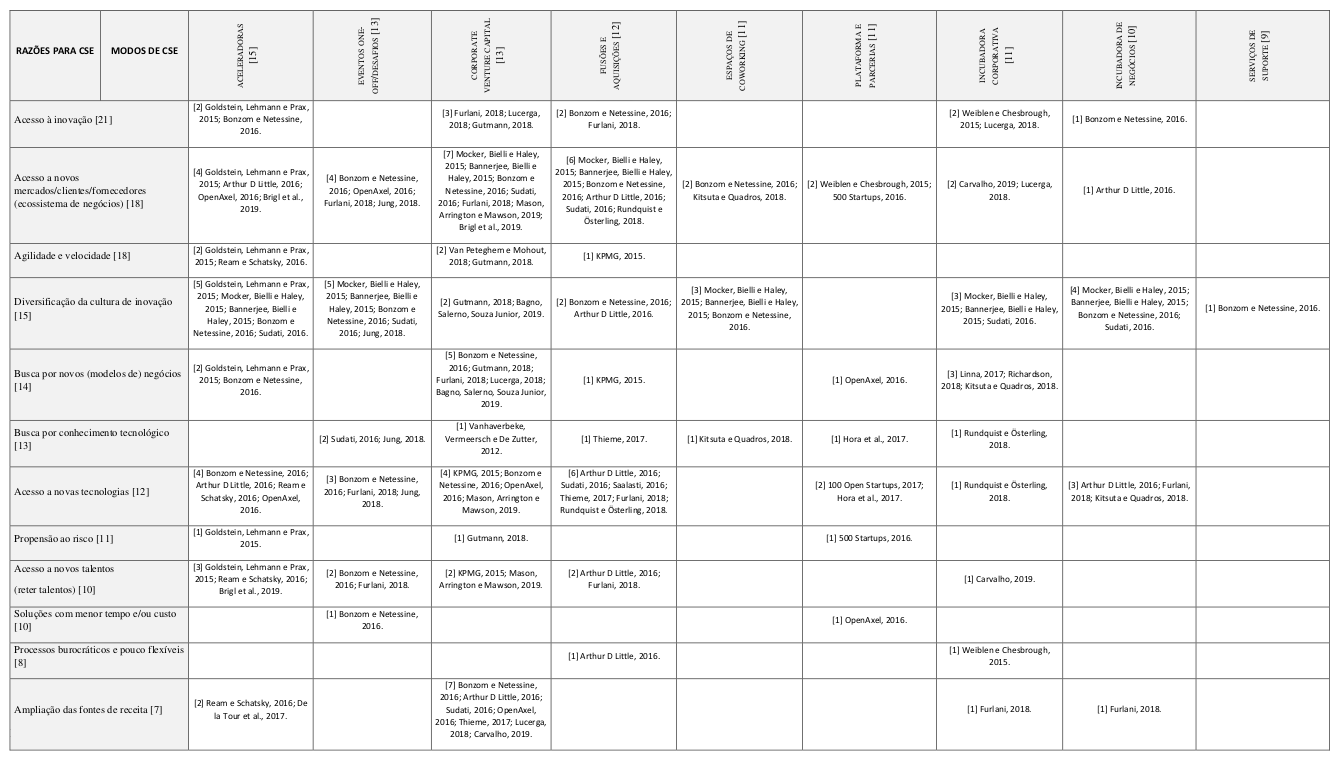
\includegraphics[width=20cm,height=15cm]{Quadros/quadro-exemplo2}}
    \source{Elaborado pelo autor}
    \label{figura-exemplo2}
  \end{figure}
\end{landscape}

And taking advantage of the quote from Satoshi Nakamoto, there are also those who say: "Bitcoin was not supposed to be like that. This is not what Satoshi Nakamoto conceived". Note, I don't know what exactly the individual or group behind the Bitcoin invention conceived. But you see, every human invention encapsulates the knowledge and knowhow of its creator. Encapsulate your ideas. But after "free in the world", invention has a "life of its own", and the ecosystem that was created from the invention has a life of its own. For good and for bad. There is not much more to be said for this.

We are near the end of the opinions I would like to express. One of the last concerns the opinions of politicians, investors, bankers and researchers about the future potential for cryptocurrencies. As I've already expressed, I see no reason to treat cryptocurrencies as an innovation unlike any other technological advance seen in humanity. And so, I am optimistic about the potential of cryptocurrencies, but realistic, far from the detachment from reality of some "moon boys". Now, one of the nuisances driving the perceived value of cryptocurrencies up is good news coming from these industries, which is fair, because it implies progress in adoption. On the other hand, there is the impact of bad news also coming from politicians, investors, bankers and researchers. And it is on this news that I want to do one of our latest mental exercises.

These people, sometimes representatives of large organizations, are ultimately the guardians of the status quo, for better or for worse. The opinions they declare, therefore, never define the true disruptive potential of cryptocurrencies, but rather the position that public opinion is wanted to believe on the subject. What do you expect to hear, for example, in an interview with, for example, an FED director? Do you think it's possible that he'll say something like: "Cryptocurrencies are indeed disruptive, they have enormous potential to transform the current financial system, and it's all a shame, because the organization I represent tends to lose more and more relevance because of it. of that and we will also lose the monopoly of issuing fiat money". Do you really think that a representative of the status quo, public or private, will say something like this? \footnote{Este é um teste para checar o correto funcionamento das notas de rodapé.}

\begin{longtable}{| p{.20\textwidth} | p{.80\textwidth} |}
\hline
foo & bar \\ \hline
foo & bar \\ \hline
foo & bar \\ \hline
foo & bar \\ \hline
foo & bar \\ \hline
foo & bar \\ \hline
foo & bar \\ \hline
foo & bar \\ \hline
foo & bar \\ \hline
foo & bar \\ \hline
foo & bar \\ \hline
\caption{Your caption here} % needs to go inside longtable environment
\label{tab:myfirstlongtable}
\end{longtable}

Representatives of the status quo will always present opinions in defense of the status quo. It doesn't matter which arguments are used. The arguments will sometimes be good, sometimes bad, but the purpose behind is always to maintain the status quo. Simultaneously with any attempt to maintain the status quo, there are organizations that perceive change as an opportunity to uplift the current status quo, that is, to turn innovation into a competitive differential for themselves. These organizations can be companies or even countries, and in the case of cryptocurrencies, they can see: "Ok, I'm going to dive into cryptocurrencies, because I can make this a competitive advantage for my country."

It is a natural scenario, inherent to any major transformation in society, markets, form and type of goods and services provided. The point is: bullish news about crypto adoption is indeed bullish news. But you have to be careful with pessimistic news, because deep down, from the beginning, you never expected anything different after all. Organizations that find themselves in a position of dominance of the current status quo, in control of the financial system, will only take positive moves in favor of cryptocurrencies to avoid a "greater evil" from falling behind in relation to other organizations that adopt cryptos as a competitive differential.

And as a last reflection, I invite you to the following reflection: how wrong can all this go? Could it be that all the disruptive potential of cryptocurrencies hasn't already been priced in, and haven't we gone much further? This question is very pertinent. The most pertinent for the cryptocurrency investor after all. The "moon boys" want us to believe that "there are no limits", but in my opinion, there is a limit. Although the adoption of cryptos by society occurs extremely quickly and painlessly, without the need for a "war" against the current status quo, even if the entire world economic system is transformed, there are still limits to the intrinsic and extrinsic value of the sector. Remember the economy is bigger than that.

Judging by the innovations that cryptocurrencies are likely to bring, I believe there is still room for investment in the sector, without it being detached from the real potential of generating value to society. And I believe this because, a lot is said about cryptoCURRENCY, but beyond that, the central point here is not the money, but the transactions. And transactions aren't just economical. Every exchange of information in social dynamics is a transaction. The combination of cryptography with a decentralized consensus protocol undoubtedly finds its greatest utility in the financial system, but it is far from being the last. Ultimately, a decentralized consensus protocol is likely to change the dynamics of the entire internet as we know it today. This is definitely not a small thing, and it is definitely not of little value.


  \chapter{Análise}
\index{Cryptocurrency}
And taking advantage of the quote from Satoshi Nakamoto, there are also those who say: "Bitcoin was not supposed to be like that. This is not what Satoshi Nakamoto conceived". Note, I don't know what exactly the individual or group behind the Bitcoin invention conceived. But you see, every human invention encapsulates the knowledge and knowhow of its creator. Encapsulate your ideas. But after "free in the world", invention has a "life of its own", and the ecosystem that was created from the invention has a life of its own. For good and for bad. There is not much more to be said for this.

We are near the end of the opinions I would like to express. One of the last concerns the opinions of politicians, investors, bankers and researchers about the future potential for cryptocurrencies. As I've already expressed, I see no reason to treat cryptocurrencies as an innovation unlike any other technological advance seen in humanity. And so, I am optimistic about the potential of cryptocurrencies, but realistic, far from the detachment from reality of some "moon boys". Now, one of the nuisances driving the perceived value of cryptocurrencies up is good news coming from these industries, which is fair, because it implies progress in adoption. On the other hand, there is the impact of bad news also coming from politicians, investors, bankers and researchers. And it is on this news that I want to do one of our latest mental exercises.

These people, sometimes representatives of large organizations, are ultimately the guardians of the status quo, for better or for worse. The opinions they declare, therefore, never define the true disruptive potential of cryptocurrencies, but rather the position that public opinion is wanted to believe on the subject. What do you expect to hear, for example, in an interview with, for example, an FED director? Do you think it's possible that he'll say something like: "Cryptocurrencies are indeed disruptive, they have enormous potential to transform the current financial system, and it's all a shame, because the organization I represent tends to lose more and more relevance because of it. of that and we will also lose the monopoly of issuing fiat money". Do you really think that a representative of the status quo, public or private, will say something like this?

Representatives of the status quo will always present opinions in defense of the status quo. It doesn't matter which arguments are used. The arguments will sometimes be good, sometimes bad, but the purpose behind is always to maintain the status quo. Simultaneously with any attempt to maintain the status quo, there are organizations that perceive change as an opportunity to uplift the current status quo, that is, to turn innovation into a competitive differential for themselves. These organizations can be companies or even countries, and in the case of cryptocurrencies, they can see: "Ok, I'm going to dive into cryptocurrencies, because I can make this a competitive advantage for my country."

\index{Bitcoin}
It is a natural scenario, inherent to any major transformation in society, markets, form and type of goods and services provided. The point is: bullish news about crypto adoption is indeed bullish news. But you have to be careful with pessimistic news, because deep down, from the beginning, you never expected anything different after all. Organizations that find themselves in a position of dominance of the current status quo, in control of the financial system, will only take positive moves in favor of cryptocurrencies to avoid a "greater evil" from falling behind in relation to other organizations that adopt cryptos as a competitive differential.

And as a last reflection, I invite you to the following reflection: how wrong can all this go? Could it be that all the disruptive potential of cryptocurrencies hasn't already been priced in, and haven't we gone much further? This question is very pertinent. The most pertinent for the cryptocurrency investor after all. The "moon boys" want us to believe that "there are no limits", but in my opinion, there is a limit. Although the adoption of cryptos by society occurs extremely quickly and painlessly, without the need for a "war" against the current status quo, even if the entire world economic system is transformed, there are still limits to the intrinsic and extrinsic value of the sector. Remember the economy is bigger than that.

Judging by the innovations that cryptocurrencies are likely to bring, I believe there is still room for investment in the sector, without it being detached from the real potential of generating value to society. And I believe this because, a lot is said about cryptoCURRENCY, but beyond that, the central point here is not the money, but the transactions. And transactions aren't just economical. Every exchange of information in social dynamics is a transaction. The combination of cryptography with a decentralized consensus protocol undoubtedly finds its greatest utility in the financial system, but it is far from being the last. Ultimately, a decentralized consensus protocol is likely to change the dynamics of the entire internet as we know it today. This is definitely not a small thing, and it is definitely not of little value.

\begin{quadro}[!hbt]
  \caption{Um quadro de exemplo}
  \begin{center}
    \begin{tabular}{ |c|c|c| }
      \hline
      cell1 & cell2 & cell3 \\
      cell4 & cell5 & cell6 \\
      cell7 & cell8 & cell9 \\
      \hline
    \end{tabular}
  \end{center}
  \source{Elaborado pelo autor}
  \label{quadro-exemplo}
\end{quadro}

And taking advantage of the quote from Satoshi Nakamoto, there are also those who say: "Bitcoin was not supposed to be like that. This is not what Satoshi Nakamoto conceived". Note, I don't know what exactly the individual or group behind the Bitcoin invention conceived. But you see, every human invention encapsulates the knowledge and knowhow of its creator. Encapsulate your ideas. But after "free in the world", invention has a "life of its own", and the ecosystem that was created from the invention has a life of its own. For good and for bad. There is not much more to be said for this.

We are near the end of the opinions I would like to express. One of the last concerns the opinions of politicians, investors, bankers and researchers about the future potential for cryptocurrencies. As I've already expressed, I see no reason to treat cryptocurrencies as an innovation unlike any other technological advance seen in humanity. And so, I am optimistic about the potential of cryptocurrencies, but realistic, far from the detachment from reality of some "moon boys". Now, one of the nuisances driving the perceived value of cryptocurrencies up is good news coming from these industries, which is fair, because it implies progress in adoption. On the other hand, there is the impact of bad news also coming from politicians, investors, bankers and researchers. And it is on this news that I want to do one of our latest mental exercises.

\index{Hathor}
These people, sometimes representatives of large organizations, are ultimately the guardians of the status quo, for better or for worse. The opinions they declare, therefore, never define the true disruptive potential of cryptocurrencies, but rather the position that public opinion is wanted to believe on the subject. What do you expect to hear, for example, in an interview with, for example, an FED director? Do you think it's possible that he'll say something like: "Cryptocurrencies are indeed disruptive, they have enormous potential to transform the current financial system, and it's all a shame, because the organization I represent tends to lose more and more relevance because of it. of that and we will also lose the monopoly of issuing fiat money". Do you really think that a representative of the status quo, public or private, will say something like this?

Representatives of the status quo will always present opinions in defense of the status quo. It doesn't matter which arguments are used. The arguments will sometimes be good, sometimes bad, but the purpose behind is always to maintain the status quo. Simultaneously with any attempt to maintain the status quo, there are organizations that perceive change as an opportunity to uplift the current status quo, that is, to turn innovation into a competitive differential for themselves. These organizations can be companies or even countries, and in the case of cryptocurrencies, they can see: "Ok, I'm going to dive into cryptocurrencies, because I can make this a competitive advantage for my country."

\begin{landscape}
  \begin{quadro}[!hbt]
    \caption{Um quadro de exemplo}
    \begin{center}
      \begin{tabular}{ |c|c|c| }
        \hline
        cell1 & cell2 & cell3 \\
        cell4 & cell5 & cell6 \\
        cell7 & cell8 & cell9 \\
        \hline
      \end{tabular}
    \end{center}
    \source{Elaborado pelo autor}
    \label{quadro-exemplo}
  \end{quadro}
\end{landscape}

It is a natural scenario, inherent to any major transformation in society, markets, form and type of goods and services provided. The point is: bullish news about crypto adoption is indeed bullish news. But you have to be careful with pessimistic news, because deep down, from the beginning, you never expected anything different after all. Organizations that find themselves in a position of dominance of the current status quo, in control of the financial system, will only take positive moves in favor of cryptocurrencies to avoid a "greater evil" from falling behind in relation to other organizations that adopt cryptos as a competitive differential.

And as a last reflection, I invite you to the following reflection: how wrong can all this go? Could it be that all the disruptive potential of cryptocurrencies hasn't already been priced in, and haven't we gone much further? This question is very pertinent. The most pertinent for the cryptocurrency investor after all. The "moon boys" want us to believe that "there are no limits", but in my opinion, there is a limit. Although the adoption of cryptos by society occurs extremely quickly and painlessly, without the need for a "war" against the current status quo, even if the entire world economic system is transformed, there are still limits to the intrinsic and extrinsic value of the sector. Remember the economy is bigger than that.

Judging by the innovations that cryptocurrencies are likely to bring, I believe there is still room for investment in the sector, without it being detached from the real potential of generating value to society. And I believe this because, a lot is said about cryptoCURRENCY, but beyond that, the central point here is not the money, but the transactions. And transactions aren't just economical. Every exchange of information in social dynamics is a transaction. The combination of cryptography with a decentralized consensus protocol undoubtedly finds its greatest utility in the financial system, but it is far from being the last. Ultimately, a decentralized consensus protocol is likely to change the dynamics of the entire internet as we know it today. This is definitely not a small thing, and it is definitely not of little value.


  \chapter{Síntese}


  \chapter{Conclusões}


  \backmatter
  %Incluir todas as referências do .bib que não foram citadas
  \nocite{*}
  \bibliographystyle{coppe-unsrt}
  \bibliography{referencias}

  \begin{appendices}
    \chapter{Cientometria}

    \chapter{Bibliometria}

Um apêndice denominado "B".
  \end{appendices}

  \printindex
\end{document}
